\begin{figure}[t!]
	\centering
	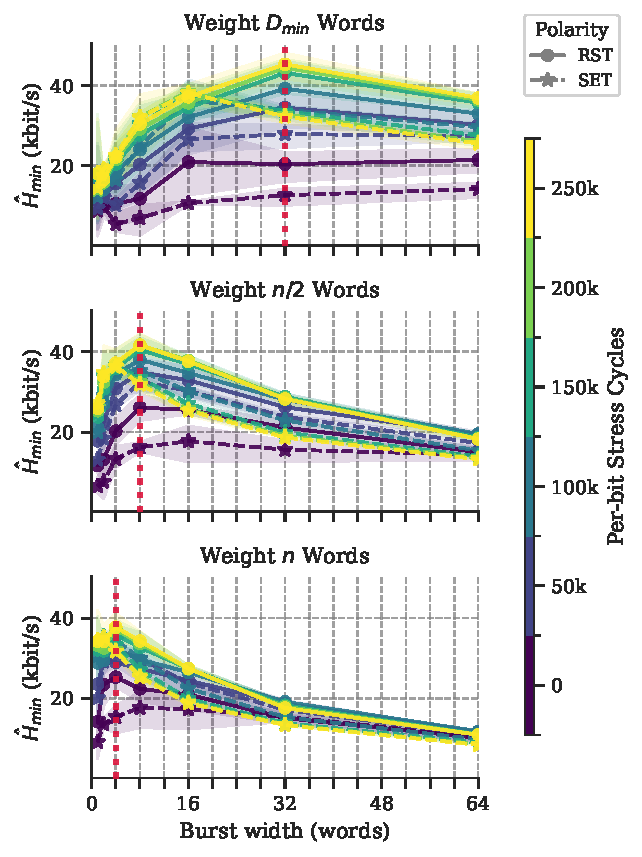
\includegraphics[width=0.49\linewidth]{img/0b_hrate_vs_bw_8m.pdf}
	\hfill
	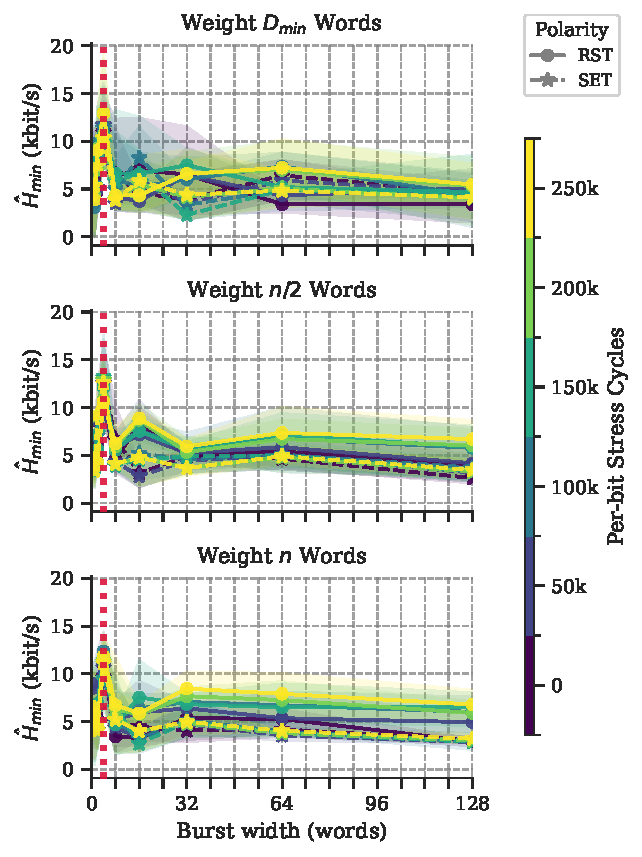
\includegraphics[width=0.50\linewidth]{img/0b_hrate_vs_bw_4m.pdf}
	\caption{
		The entropy rate measured over various wear-leveled codeword sequence compositions and burst sizes for 3  MB85AS4MT 4Mb (right) and 3 MB85AS8MT 8Mb (left) modules from Ramxeed under varying stress levels.
		Each codeword composition is defined by the number of active transitioning bits.
		Several passes are conducted with a uniform stress sequence conducted after each measurement period.
		For the 8M peaks in entropy efficiency are distinguishable at at burst length 32, 8, and 4, for $D_{min}$, $n//2$, and $n$ weight codewords, respectively.
		For the 4M peaks in entropy efficiency are distinguishable at at burst length 4, for $D_{min}$, $n//2$, and $n$ weight codewords.
		\label{fig:opt-burst8m}
	}
\end{figure}